\documentclass{IEEEtran}
\usepackage[utf8]{vietnam}

\usepackage{cite}
\usepackage{amsmath,amssymb,amsfonts}
\usepackage{graphicx}
\usepackage{textcomp,nicefrac}
\usepackage{multirow}
\usepackage{tikz}
\usetikzlibrary{arrows.meta,calc}
\def\BibTeX{{\rm B\kern-.05em{\sc i\kern-.025em b}\kern-.08em
T\kern-.1667em\lower.7ex\hbox{E}\kern-.125emX}}
\markboth{STUDENT SCIENTIFIC RESEARCH COMMUNICATION, Volume II, 2026}
{Nguyễn Ngọc Minh \MakeLowercase{\textit{et al.}}: Grounding Recipe Steps in Long Instructional Videos}
\begin{document}
\title{Grounding Recipe Steps in Long Instructional Videos with Audio-Visual Multi-Task Learning and LLM Distillation}
\author{Nguyễn Ngọc Minh, Phan Công Chiến, and Trần Nhật Hoàng Anh
\thanks{Bản thảo nộp ngày \ldots/\ldots/2026, bản chỉnh sửa nộp ngày \ldots/\ldots/2026. Nghiên cứu được thực hiện trong khuôn khổ khoá luận tốt nghiệp tại Khoa Công nghệ Thông tin, Trường Đại học Công nghiệp TP. Hồ Chí Minh. (Điền thông tin tài trợ nếu có; nếu không, ghi: ``Nghiên cứu không nhận tài trợ từ tổ chức nào.'')}
\thanks{Nguyễn Ngọc Minh và Phan Công Chiến là sinh viên Khoa Công nghệ Thông tin, Trường Đại học Công nghiệp TP. Hồ Chí Minh, 12 Nguyễn Văn Bảo, TP. Hồ Chí Minh, Việt Nam (e-mail: \ldots; \ldots). Hai tác giả đóng góp như nhau cho việc xây dựng mô hình, chạy thực nghiệm và viết bài.}
\thanks{ThS. Trần Nhật Hoàng Anh, giảng viên hướng dẫn, công tác tại Khoa Công nghệ Thông tin, Trường Đại học Công nghiệp TP. Hồ Chí Minh, 12 Nguyễn Văn Bảo, TP. Hồ Chí Minh, Việt Nam (e-mail: \ldots). Tác giả liên hệ: \ldots.}}

\maketitle

\begin{abstract}
Instructional videos are often long, and only a small fraction of each video shows the steps of the task, so viewers need to know where every step starts and ends. This paper presents a multi-task audio-visual model that solves \emph{three tasks} on the HT-Step dataset: localizing the steps of a recipe in a video, recognizing which recipe the video follows, and producing for every localized segment a multimodal embedding of its content. The model builds on precomputed visual and audio features and a two-stream audio-visual backbone with a multi-scale temporal pyramid, so that both short and long steps can be detected. The multimodal embedding is learned by distillation from a \emph{seven-billion-parameter} audio-visual retrieval model. Distillation teaches our model, which has only 137 million parameters, about fifty times fewer, to reproduce these embeddings from the features it already computes, through a point-wise and a segment-wise head. On the validation split of seen activities, the model reaches a mean average precision of 30.98 for step localization, recognizes the correct recipe for 59.8\% of the videos, and reaches a mean-centered cosine similarity of 0.660 with the embeddings of the large model.

Instructional video thường dài, và chỉ một phần nhỏ thời lượng của mỗi video thể hiện các bước thực hiện, nên người xem cần biết mỗi bước bắt đầu và kết thúc ở đâu. Bài báo trình bày một multi-task audio-visual model giải quyết \emph{ba nhiệm vụ} trên bộ dữ liệu HT-Step: step localization (định vị các bước của một recipe trong video), recipe recognition (nhận biết video đang làm theo recipe nào), và tạo cho mỗi segment được định vị một multimodal embedding biểu diễn nội dung của segment đó. Mô hình dựa trên các visual feature và audio feature được trích sẵn, cùng một two-stream audio-visual backbone với multi-scale temporal pyramid, nhờ đó phát hiện được cả những bước ngắn lẫn những bước dài. Multimodal embedding được học bằng knowledge distillation từ một audio-visual retrieval model \emph{bảy tỉ tham số}. Distillation dạy mô hình của chúng tôi, chỉ có 137 triệu tham số, tức nhỏ hơn khoảng năm mươi lần, tái tạo các embedding này từ chính những feature mà nó đã tính, thông qua một point-wise head và một segment-wise head. Trên validation split của các seen activity, mô hình đạt mean average precision 30,98 cho step localization, nhận biết đúng recipe cho 59,8\% số video, và đạt mean-centered cosine similarity 0,660 so với embedding của mô hình lớn.
\end{abstract}

\begin{IEEEkeywords}
Audio-visual learning, HT-Step, knowledge distillation, multimodal embedding, step localization.
\end{IEEEkeywords}

\begin{figure*}[t]
\centering
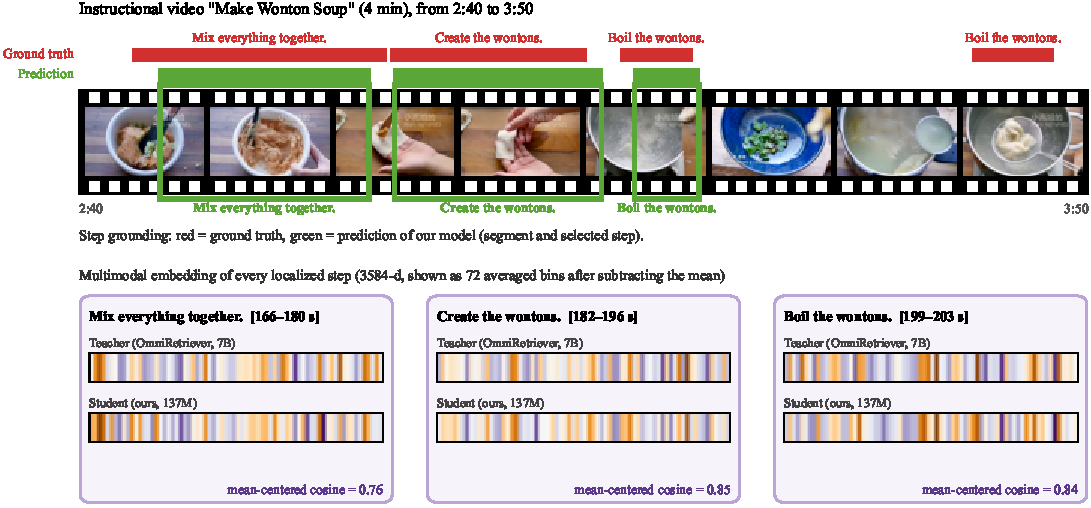
\includegraphics[width=\textwidth]{fig_teaser.pdf}
\begin{minipage}{0.86\textwidth}
\caption{Ví dụ trên một video của tập val\_seen (``Make Wonton Soup'', 4 phút). \emph{Hàng trên}: đoạn từ 2:40 đến 3:50, nơi chứa các bước của recipe; thanh \textcolor{red}{đỏ} là đoạn ground truth kèm tên bước, thanh và khung \textcolor{green!50!black}{xanh} là đoạn mô hình dự đoán kèm bước được chọn. Mô hình định vị đúng ba đoạn (IoU 0,83; 0,91; 0,73) và chọn đúng bước cho cả ba, nhưng bỏ sót lần ``Boil the wontons'' thứ hai ở cuối video. \emph{Hàng dưới}: embedding 3584 chiều của từng đoạn, do teacher OmniRetriever (7 tỉ tham số) và do mô hình của chúng tôi (137 triệu tham số) tạo ra; để dễ nhìn, mỗi embedding được trừ trung bình rồi gộp thành 72 ô. Hai embedding có mean-centered cosine từ 0,76 đến 0,85.}
\label{fig:teaser}
\end{minipage}
\end{figure*}

\section{Giới thiệu}
\label{sec:introduction}
\IEEEPARstart{V}{ideo} hướng dẫn trên mạng là nguồn học kỹ năng phổ biến, nhưng một video nấu ăn thường dài hàng chục phút, trong đó phần lớn thời lượng là lời giới thiệu, chuẩn bị hay trò chuyện. Bộ dữ liệu HT-Step~\cite{htstep} gán nhãn thời gian cho các bước của bài viết hướng dẫn (article) trên các video của HowTo100M~\cite{howto100m}; các đoạn được gán nhãn chỉ phủ khoảng 20\% độ dài video. Bài toán \emph{article grounding} của HT-Step yêu cầu: cho một video và recipe của nó, tìm vị trí thời gian của từng bước trong recipe (Hình~\ref{fig:teaser}).

Bài toán khó vì ba lý do. Thứ nhất, cùng một bước như ``đập trứng vào bát'' có thể dài vài giây hoặc vài phút, nên mô hình cần nhìn video ở nhiều độ phân giải thời gian. Thứ hai, các bước của cùng một recipe trông rất giống nhau, nên việc gán đúng bước cho một đoạn đòi hỏi hiểu cả hình ảnh lẫn văn bản. Thứ ba, ở các ứng dụng retrieval, mỗi đoạn tìm được còn cần một vector mô tả để so với câu truy vấn; các mô hình đa phương thức lớn cho vector tốt nhưng quá chậm để chạy trên mọi đoạn của mọi video.

Các nghiên cứu gần đây như OmniRetriever~\cite{omniretriever} đạt kết quả rất cao trong text-to-video retrieval, nhưng chỉ làm việc trên các đoạn đã cắt sẵn, mỗi đoạn một step, và với hàng tỉ tham số thì quá tốn kém để chạy trên mọi đoạn của mọi video. Ngược lại, các mô hình temporal localization như ActionFormer~\cite{actionformer} trích xuất được các step từ một untrimmed video mà vẫn nhỏ gọn.

Từ đó, chúng tôi kết hợp kiến trúc của ActionFormer để định vị các step với teacher--student distillation để distill tri thức từ OmniRetriever. Mỗi step được định vị nhờ vậy có một embedding trong không gian của OmniRetriever, sẵn sàng cho text-based retrieval, mà không cần huấn luyện lại hay chạy mô hình hàng tỉ tham số.

Bài báo đề xuất một multi-task model theo hướng ActionFormer~\cite{actionformer}, mở rộng thành hai luồng audio-visual, và giải đồng thời cả ba việc. Các đóng góp chính gồm:
\begin{itemize}
\item Một mô hình step localization theo hướng ActionFormer~\cite{actionformer} có conditioning theo văn bản các bước của recipe, kèm một recipe head và một step classification head cho mỗi đoạn.
\item Một cách distill embedding của audio-visual retrieval model bảy tỉ tham số vào một point-wise head và một segment-wise head, với cosine loss đã trừ trung bình để khớp với thang đo.
\item Một ridge regression trên input feature, ghép lúc inference, tăng similarity với teacher embedding từ 66,01 lên 73,86 mà không cần huấn luyện lại.
\item Một loạt ablation và phân tích upper bound, cho biết thành phần nào có ích và giới hạn còn lại nằm ở đâu.
\end{itemize}

\section{Công trình liên quan}
\textbf{Temporal action localization.} Các phương pháp hai giai đoạn như BMN~\cite{bmn} và G-TAD~\cite{gtad} sinh proposal rồi mới phân loại. ActionFormer~\cite{actionformer} gộp thành một giai đoạn: tại mỗi điểm của một feature pyramid, mô hình dự đoán trực tiếp xác suất có sự kiện và khoảng cách tới hai biên. Bài báo HT-Step~\cite{htstep} dùng ActionFormer làm mô hình cơ sở và đề xuất ActionFormer-T, có thêm văn bản các bước làm điều kiện. UniAV~\cite{uniav} mở rộng khung này thành hai luồng hình ảnh và âm thanh có cross-attention.

\textbf{Step grounding trong instructional video.} VINA~\cite{vina} học từ lời thuyết minh thay cho nhãn thời gian. BaGLM~\cite{baglm} và HSD~\cite{hsd} là các phương pháp training-free, dùng trực tiếp một mô hình đa phương thức lớn và xử lý video theo luồng. Các cách này không cần nhãn nhưng độ chính xác định vị còn kém xa cách supervised.

\textbf{Video--text retrieval.} CLIP~\cite{clip} và CLIP4Clip~\cite{clip4clip} học một không gian chung cho hình ảnh và văn bản bằng contrastive learning. OmniRetriever~\cite{omniretriever}, dựa trên WAVE~\cite{wave}, dùng một mô hình bảy tỉ tham số để đưa video, âm thanh và văn bản vào cùng một không gian 3584 chiều, nhưng chỉ làm việc trên các đoạn đã cắt sẵn.

\textbf{Knowledge distillation.} Knowledge distillation~\cite{kd} dạy một student nhỏ bắt chước một teacher lớn; relational knowledge distillation~\cite{rkd} cho student học quan hệ giữa các mẫu. Với embedding, InfoNCE loss~\cite{infonce} thường được dùng, và MoCo~\cite{moco} dùng một hàng đợi negative từ các batch trước. Chúng tôi kết hợp các ý tưởng này để distill embedding của OmniRetriever vào một mô hình step localization nhỏ.

\section{Phương pháp}

\subsection{Dữ liệu vào và bài toán}
Với mỗi video và danh sách các bước của recipe, mô hình tìm đoạn $(t_s, t_e)$ của từng bước. Đồng thời, mô hình đoán recipe của video và tạo cho mỗi đoạn một embedding $\hat{\mathbf{s}} \in \mathbb{R}^{3584}$ gần với teacher embedding $\mathbf{t}$ của đoạn đó.

Mọi feature được trích sẵn từ trước bằng các mô hình đã huấn luyện:
\begin{itemize}
\item \emph{Visual feature}: mỗi giây một vector 768 chiều từ InternVideo2~\cite{internvideo2} tinh chỉnh trên Kinetics-400.
\item \emph{Audio feature}: mỗi giây một vector 768 chiều từ BEATs~\cite{beats}.
\item \emph{Văn bản các bước}: mỗi bước trong 4958 bước được mã hoá bằng text encoder của InternVideo2 thành một vector 512 chiều.
\item \emph{Teacher embedding}: với mỗi đoạn GT, OmniRetriever~\cite{omniretriever} nhận khung hình và âm thanh của đoạn, trả về một embedding 3584 chiều.
\end{itemize}

\subsection{Backbone audio-visual}
Mô hình theo khung của ActionFormer~\cite{actionformer}; backbone gồm hai luồng hình ảnh và âm thanh có cross-attention giữa hai luồng như UniAV~\cite{uniav}. Mỗi luồng đi qua hai lớp tích chập, ba khối transformer ở độ phân giải gốc, rồi năm khối transformer có giảm mẫu hai lần sau mỗi khối, tạo temporal pyramid sáu tầng với bước nhảy $1, 2, \ldots, 32$. Ở mỗi tầng, hai luồng trao đổi thông tin qua cross-attention. Feature của hai luồng (mỗi luồng 512 kênh) được nối lại thành $\mathbf{F}_l \in \mathbb{R}^{1024 \times T_l}$, tổng cộng $P = 504$ điểm trên sáu tầng (Hình~\ref{fig:backbone}).

\begin{figure}[t]
\centering
\resizebox{\columnwidth}{!}{% Audio-visual backbone (two streams, cross-attention, six-level temporal pyramid)
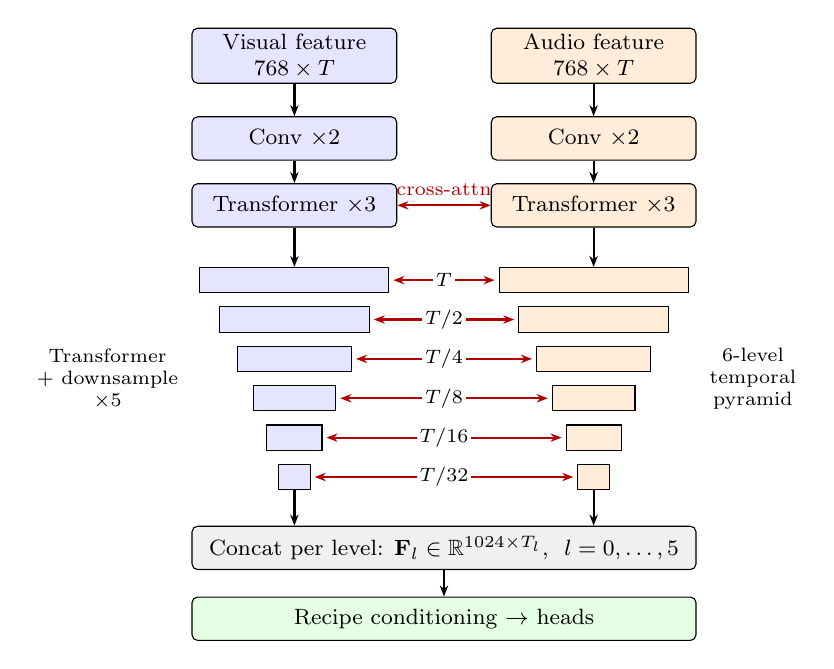
\begin{tikzpicture}[
  font=\footnotesize,
  box/.style={draw, rounded corners=2pt, minimum height=0.55cm, align=center, inner sep=2pt},
  vis/.style={box, fill=blue!10, minimum width=2.6cm},
  aud/.style={box, fill=orange!15, minimum width=2.6cm},
  catbox/.style={box, fill=gray!12, minimum width=6.4cm},
  arr/.style={-{Stealth[length=4pt]}, thick},
  xatt/.style={{Stealth[length=4pt]}-{Stealth[length=4pt]}, thick, red!70!black},
]
% inputs
\node[vis] (vin) at (-1.9, 0) {Visual feature\\$768 \times T$};
\node[aud] (ain) at ( 1.9, 0) {Audio feature\\$768 \times T$};
% stem
\node[vis] (vc) at (-1.9,-1.05) {Conv $\times 2$};
\node[aud] (ac) at ( 1.9,-1.05) {Conv $\times 2$};
\node[vis] (vt) at (-1.9,-1.9) {Transformer $\times 3$};
\node[aud] (at) at ( 1.9,-1.9) {Transformer $\times 3$};
\draw[arr] (vin) -- (vc); \draw[arr] (vc) -- (vt);
\draw[arr] (ain) -- (ac); \draw[arr] (ac) -- (at);
\draw[xatt] (vt) -- node[above, font=\scriptsize] {cross-attn} (at);

% temporal pyramid: 6 levels, length halves at every level
\foreach \l/\w/\lab in {0/2.4/{T}, 1/1.9/{T/2}, 2/1.45/{T/4}, 3/1.05/{T/8}, 4/0.7/{T/16}, 5/0.4/{T/32}} {
  \pgfmathsetmacro{\y}{-2.85 - 0.5*\l}
  \node[draw, fill=blue!10, minimum width=\w cm, minimum height=0.32cm, inner sep=0pt] (v\l) at (-1.9, \y) {};
  \node[draw, fill=orange!15, minimum width=\w cm, minimum height=0.32cm, inner sep=0pt] (a\l) at ( 1.9, \y) {};
  \draw[xatt] (v\l.east) ++(0.05,0) -- ($(a\l.west)+(-0.05,0)$);
  \node[font=\scriptsize, fill=white, inner sep=1pt] at (0, \y) {$\lab$};
}
\draw[arr] (vt) -- (v0); \draw[arr] (at) -- (a0);
\node[font=\scriptsize, align=center, anchor=east] at (-3.25,-4.1) {Transformer\\+ downsample\\$\times 5$};
\node[font=\scriptsize, align=center, anchor=west] at ( 3.25,-4.1) {6-level\\temporal\\pyramid};

% concat and output
\node[catbox] (cat) at (0,-6.25) {Concat per level: $\mathbf{F}_l \in \mathbb{R}^{1024 \times T_l}$, \ $l = 0,\ldots,5$};
\draw[arr] (v5) -- (v5 |- cat.north); \draw[arr] (a5) -- (a5 |- cat.north);
\node[catbox, fill=green!10] (heads) at (0,-7.15) {Recipe conditioning $\rightarrow$ heads};
\draw[arr] (cat) -- (heads);
\end{tikzpicture}
}
\caption{Backbone audio-visual. Hai chuỗi feature đầu vào (visual feature từ InternVideo2 và audio feature từ BEATs, mỗi chuỗi $768 \times T$ với $T = 256$) được xử lý bởi hai luồng riêng có cùng cấu trúc: hai lớp Conv1D để chiếu feature về 512 kênh, ba khối transformer ở độ phân giải gốc, rồi năm khối transformer, mỗi khối giảm độ dài chuỗi đi một nửa. Kết quả là một temporal pyramid sáu tầng với độ dài $T, T/2, \ldots, T/32$: tầng mịn phù hợp với các bước ngắn, tầng thô phù hợp với các bước dài. Ở mỗi tầng, hai luồng trao đổi thông tin qua cross-attention (mũi tên đỏ), để âm thanh bổ sung cho hình ảnh và ngược lại. Cuối cùng, feature của hai luồng được nối lại thành $\mathbf{F}_l$ có 1024 kênh ở mỗi tầng $l$, làm đầu vào cho recipe conditioning và các head.}
\label{fig:backbone}
\end{figure}

\subsection{Recipe conditioning}
Theo ý tưởng của ActionFormer-T~\cite{htstep}, feature ở mọi tầng được chú ý tới văn bản các bước của recipe. Gọi $\mathbf{E} \in \mathbb{R}^{C \times 512}$ là vector văn bản của $C$ bước. Với mỗi tầng,
\begin{equation}
\label{eq:artc}
\mathbf{F}'_l = \mathbf{F}_l + \mathrm{MHA}\big(\mathrm{LN}(\mathbf{F}_l),\ \mathbf{K},\ \mathbf{K}\big), \quad \mathbf{K} = \mathrm{LN}(\mathbf{E}\mathbf{W}) + \mathbf{O},
\end{equation}
trong đó $\mathbf{O}$ là embedding vị trí của bước trong recipe. Lớp chiếu ra của khối chú ý được khởi tạo bằng 0, nên lúc đầu khối này không làm thay đổi feature. Cùng một khối (chung trọng số) được dùng cho cả sáu tầng (Hình~\ref{fig:recipecond}).

\begin{figure}[t]
\centering
\resizebox{\columnwidth}{!}{% Recipe conditioning: the features of every pyramid level attend to the texts of the recipe steps
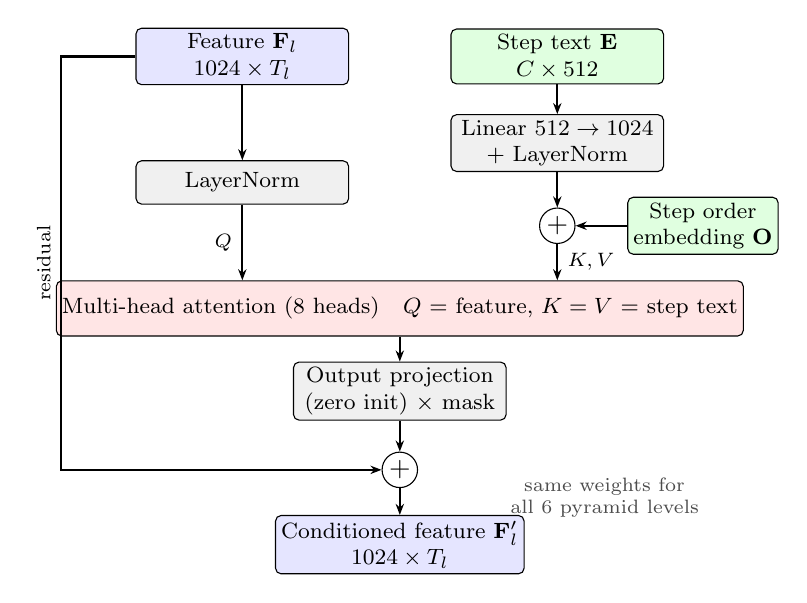
\begin{tikzpicture}[
  font=\footnotesize,
  box/.style={draw, rounded corners=2pt, minimum height=0.55cm, align=center, inner sep=2pt},
  feat/.style={box, fill=blue!10, minimum width=2.7cm},
  txt/.style={box, fill=green!12, minimum width=2.7cm},
  op/.style={box, fill=gray!12, minimum width=2.7cm},
  arr/.style={-{Stealth[length=4pt]}, thick},
  sum/.style={draw, circle, inner sep=0pt, minimum size=0.45cm, font=\normalsize},
]
% inputs
\node[feat] (f) at (-2, 0) {Feature $\mathbf{F}_l$\\$1024 \times T_l$};
\node[txt]  (e) at ( 2, 0) {Step text $\mathbf{E}$\\$C \times 512$};

% text branch: keys / values
\node[op] (lin) at (2,-1.1) {Linear $512 \rightarrow 1024$\\+ LayerNorm};
\node[sum] (plus) at (2,-2.15) {$+$};
\node[txt, minimum width=1.9cm] (ord) at (3.85,-2.15) {Step order\\embedding $\mathbf{O}$};
\draw[arr] (e) -- (lin); \draw[arr] (lin) -- (plus); \draw[arr] (ord) -- (plus);

% feature branch: queries
\node[op] (ln) at (-2,-1.6) {LayerNorm};
\draw[arr] (f) -- (ln);

% attention
\node[box, fill=red!10, minimum width=6.7cm, minimum height=0.7cm] (mha) at (0,-3.2)
  {Multi-head attention (8 heads)\quad $Q$ = feature,\ $K = V$ = step text};
\draw[arr] (ln) -- node[left, font=\scriptsize] {$Q$} (ln |- mha.north);
\draw[arr] (plus) -- node[right, font=\scriptsize] {$K, V$} (plus |- mha.north);

\node[op] (proj) at (0,-4.25) {Output projection\\(zero init) $\times$ mask};
\draw[arr] (mha) -- (proj);

% residual
\node[sum] (res) at (0,-5.25) {$+$};
\draw[arr] (proj) -- (res);
\draw[arr] (f.west) -- ++(-0.95,0) |- node[pos=0.25, rotate=90, above, font=\scriptsize] {residual} (res.west);

\node[feat] (out) at (0,-6.2) {Conditioned feature $\mathbf{F}'_l$\\$1024 \times T_l$};
\draw[arr] (res) -- (out);

\node[font=\scriptsize, align=center, text=gray!60!black] at (2.6,-5.6) {same weights for\\all 6 pyramid levels};
\end{tikzpicture}
}
\caption{Recipe conditioning. Văn bản các bước của recipe ($C$ bước, mỗi bước một vector 512 chiều) được chiếu lên 1024 chiều, chuẩn hoá bằng LayerNorm và cộng với embedding thứ tự của bước trong recipe, tạo thành key và value. Feature $\mathbf{F}_l$ của mỗi tầng, sau LayerNorm, đóng vai trò query. Nhờ multi-head attention (8 head), mỗi thời điểm trong video tìm những bước của recipe giống nó nhất và lấy thông tin từ các bước đó. Kết quả qua một lớp chiếu ra, nhân với mask để bỏ các vị trí padding, rồi được cộng residual vào $\mathbf{F}_l$, cho feature $\mathbf{F}'_l$. Lớp chiếu ra được khởi tạo bằng 0, nên lúc bắt đầu huấn luyện khối này chưa làm thay đổi feature và chỉ dần học cách dùng văn bản. Cùng một khối được dùng cho cả sáu tầng của pyramid.}
\label{fig:recipecond}
\end{figure}

\subsection{Localization head và step classification}
Hình~\ref{fig:heads} cho cấu trúc bên trong của các head chính. Trên $\mathbf{F}'_l$, ba convolutional head dùng chung trọng số giữa các tầng:
\begin{itemize}
\item Event head cho xác suất điểm nằm trong một bước, học bằng focal loss~\cite{focal}.
\item Boundary head cho khoảng cách tới hai biên của bước, học bằng DIoU loss~\cite{diou}, kèm một điểm chất lượng IoU để xếp hạng.
\item Embedding head cho mỗi điểm một vector 512 chiều, học bằng InfoNCE so với vector văn bản các bước.
\end{itemize}
Lúc inference, điểm của một đoạn là tích của xác suất sự kiện và điểm chất lượng; các đoạn được gộp bằng soft-NMS.

Để chọn bước cho một đoạn, khối \emph{SegmentContext} gộp feature tầng 0 trong đoạn bằng attention pooling, ghép thêm trung bình cả video và vị trí tương đối của đoạn, rồi qua một MLP. Vector thu được được so cosine với văn bản các bước của recipe, và bước có điểm cao nhất được chọn.

\begin{figure*}[t]
\centering
\resizebox{\textwidth}{!}{% Inside the main heads (libs/modeling/heads.py): localization (event, boundary) and distillation (point-wise, segment-wise)
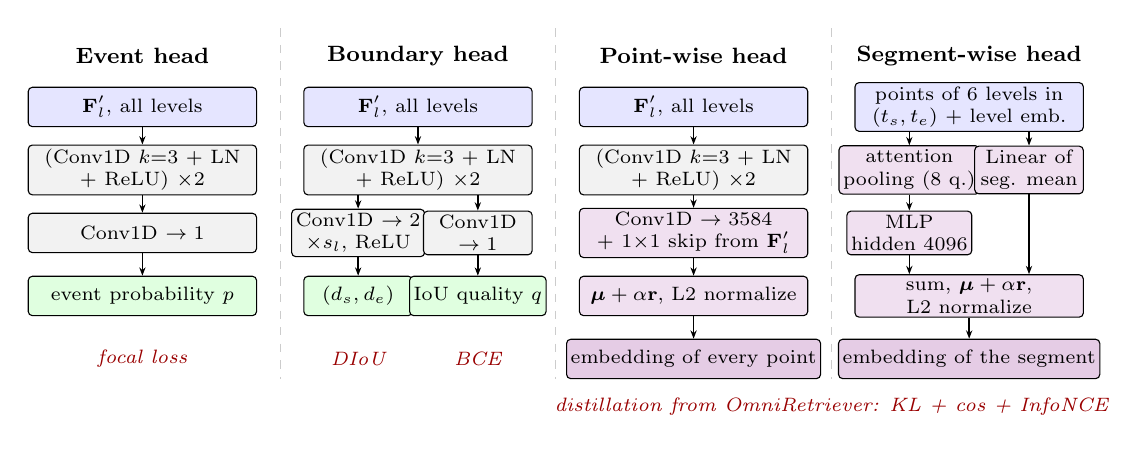
\begin{tikzpicture}[
  font=\scriptsize,
  layer/.style={draw, rounded corners=1.5pt, fill=gray!10, minimum width=2.9cm, minimum height=0.5cm, align=center, inner sep=1.5pt},
  half/.style={layer, minimum width=1.38cm},
  inp/.style={layer, fill=blue!10},
  title/.style={font=\footnotesize\bfseries, align=center},
  outp/.style={layer, fill=green!12},
  omni/.style={layer, fill=violet!12},
  loss/.style={font=\scriptsize\itshape, text=red!60!black, align=center},
  arr/.style={-{Stealth[length=3pt]}, semithick},
]
\def\ya{0}      % title
\def\yb{-0.65}  % input
\def\yc{-1.45}
\def\yd{-2.25}
\def\ye{-3.05}
\def\yf{-3.85}

% ---------------- Event head ----------------
\begin{scope}[xshift=0cm]
\node[title] at (0,\ya) {Event head};
\node[inp] (a1) at (0,\yb) {$\mathbf{F}'_l$, all levels};
\node[layer] (a2) at (0,\yc) {(Conv1D $k{=}3$ + LN\\+ ReLU) $\times 2$};
\node[layer] (a3) at (0,\yd) {Conv1D $\rightarrow 1$};
\node[outp] (a4) at (0,\ye) {event probability $p$};
\draw[arr] (a1)--(a2); \draw[arr] (a2)--(a3); \draw[arr] (a3)--(a4);
\node[loss] at (0,\yf) {focal loss};
\end{scope}

% ---------------- Boundary head ----------------
\begin{scope}[xshift=3.5cm]
\node[title] at (0,\ya) {Boundary head};
\node[inp] (b1) at (0,\yb) {$\mathbf{F}'_l$, all levels};
\node[layer] (b2) at (0,\yc) {(Conv1D $k{=}3$ + LN\\+ ReLU) $\times 2$};
\node[half] (b3) at (-0.76,\yd) {Conv1D $\rightarrow 2$\\$\times s_l$, ReLU};
\node[half] (b4) at ( 0.76,\yd) {Conv1D\\$\rightarrow 1$};
\node[outp, minimum width=1.38cm] (b5) at (-0.76,\ye) {$(d_s, d_e)$};
\node[outp, minimum width=1.38cm] (b6) at ( 0.76,\ye) {IoU quality $q$};
\draw[arr] (b1)--(b2); \draw[arr] (b2.south -| b3)--(b3); \draw[arr] (b2.south -| b4)--(b4);
\draw[arr] (b3)--(b5); \draw[arr] (b4)--(b6);
\node[loss] at (-0.76,\yf) {DIoU}; \node[loss] at (0.76,\yf) {BCE};
\end{scope}

% ---------------- Point-wise head ----------------
\begin{scope}[xshift=7.0cm]
\node[title] at (0,\ya) {Point-wise head};
\node[inp] (c1) at (0,\yb) {$\mathbf{F}'_l$, all levels};
\node[layer] (c2) at (0,\yc) {(Conv1D $k{=}3$ + LN\\+ ReLU) $\times 2$};
\node[omni] (c3) at (0,\yd) {Conv1D $\rightarrow 3584$\\+ $1{\times}1$ skip from $\mathbf{F}'_l$};
\node[omni] (c4) at (0,\ye) {$\boldsymbol{\mu} + \alpha\mathbf{r}$, L2 normalize};
\node[outp, fill=violet!20] (c5) at (0,\yf) {embedding of every point};
\draw[arr] (c1)--(c2); \draw[arr] (c2)--(c3); \draw[arr] (c3)--(c4); \draw[arr] (c4)--(c5);
\end{scope}

% ---------------- Segment-wise head ----------------
\begin{scope}[xshift=10.5cm]
\node[title] at (0,\ya) {Segment-wise head};
\node[inp] (e1) at (0,\yb) {points of 6 levels in\\$(t_s, t_e)$ + level emb.};
\node[half, fill=violet!12] (e2) at (-0.76,\yc) {attention\\pooling (8 q.)};
\node[half, fill=violet!12] (e3) at ( 0.76,\yc) {Linear of\\seg. mean};
\node[half, fill=violet!12] (e4) at (-0.76,\yd) {MLP\\hidden 4096};
\node[omni] (e5) at (0,\ye) {sum, $\boldsymbol{\mu} + \alpha\mathbf{r}$,\\L2 normalize};
\node[outp, fill=violet!20] (e6) at (0,\yf) {embedding of the segment};
\draw[arr] (e1.south -| e2)--(e2); \draw[arr] (e1.south -| e3)--(e3); \draw[arr] (e2)--(e4);
\draw[arr] (e4.south)--(e4.south |- e5.north); \draw[arr] (e3.south)--(e3.south |- e5.north);
\draw[arr] (e5)--(e6);
\end{scope}

% shared distillation loss of the two embedding heads
\node[loss] at (8.75,\yf-0.6) {distillation from OmniRetriever: KL + cos + InfoNCE};

% separators
\foreach \x in {1.75, 5.25, 8.75} { \draw[gray!40, dashed] (\x, 0.35) -- (\x, -4.1); }
\end{tikzpicture}
}
\caption{Cấu trúc bên trong của các head chính. \emph{Event head} và \emph{boundary head} là hai localization head, chạy trên feature $\mathbf{F}'_l$ của mọi tầng với trọng số dùng chung. Mỗi head có hai lớp Conv1D (kernel 3) kèm LayerNorm và ReLU; event head kết thúc bằng một Conv1D cho xác suất $p$ rằng điểm đó nằm trong một bước, còn boundary head tách thành hai nhánh: một nhánh cho khoảng cách $(d_s, d_e)$ từ điểm đó tới hai biên của bước (nhân với hệ số $s_l$ học được của từng tầng), một nhánh cho điểm chất lượng $q$ ước lượng IoU giữa đoạn dự đoán và đoạn thật. \emph{Point-wise head} và \emph{segment-wise head} (màu tím) được distill từ OmniRetriever. Point-wise head cho mỗi điểm một embedding 3584 chiều, qua một Conv1D cộng với nhánh skip $1{\times}1$ từ $\mathbf{F}'_l$. Segment-wise head biết trước thời điểm đầu và cuối của đoạn, gom mọi điểm của sáu tầng nằm trong đoạn (cộng embedding của tầng), rồi tạo một embedding cho cả đoạn bằng attention pooling với 8 query và MLP, song song với một nhánh tuyến tính trên trung bình các điểm. Cả hai head chỉ dự đoán phần lệch $\mathbf{r}$ quanh trung bình $\boldsymbol{\mu}$ của các teacher embedding, rồi chuẩn hoá L2. Chữ đỏ in nghiêng là loss của mỗi đầu ra.}
\label{fig:heads}
\end{figure*}

\subsection{Recipe head}
Recipe head dùng feature \emph{trước} khi conditioning, vì feature sau~\eqref{eq:artc} đã chứa văn bản của recipe đúng. Vector video $\mathbf{v}$ là MLP của trung bình và max theo thời gian của feature tầng 0. Vector của recipe $a$ là $\mathbf{u}_a = \mathbf{W}_t \bar{\mathbf{e}}_a + \mathbf{b}_a$, với $\bar{\mathbf{e}}_a$ là trung bình văn bản các bước của nó và $\mathbf{b}_a$ là một vector học được, khởi tạo bằng 0. Điểm của recipe là cosine giữa $\mathbf{v}$ và $\mathbf{u}_a$ nhân với một nhiệt độ học được; head này học bằng cross-entropy trên 617 recipe.

\subsection{Distillation cho multimodal embedding}
Teacher embedding $\mathbf{t}$ (đã chuẩn hoá L2) là vector mà OmniRetriever tính cho từng đoạn GT, từ 8 khung hình và âm thanh của đoạn. Hai student head dự đoán vector này:
\begin{itemize}
\item \emph{Point-wise head}: một nhánh của embedding head, cho mỗi điểm nằm trong một đoạn GT một vector 3584 chiều.
\item \emph{Segment-wise head}: biết trước thời điểm đầu và cuối của đoạn, lấy mọi điểm của sáu tầng nằm trong đoạn, cộng embedding của tầng, rồi gộp bằng attention pooling với 8 truy vấn và một MLP ẩn 4096 chiều. Một nhánh tuyến tính trên trung bình các điểm trong đoạn được cộng song song.
\end{itemize}
Phần mà mọi teacher embedding cùng có rất lớn: chỉ cần dự đoán trung bình $\boldsymbol{\mu}$ của các teacher embedding trên tập huấn luyện đã được cosine khoảng 0,80. Vì vậy cả hai head dự đoán phần lệch quanh $\boldsymbol{\mu}$:
\begin{equation}
\label{eq:dev}
\hat{\mathbf{s}} = \frac{\boldsymbol{\mu} + \alpha\,\mathbf{r}}{\lVert \boldsymbol{\mu} + \alpha\,\mathbf{r} \rVert},
\end{equation}
trong đó $\mathbf{r}$ là đầu ra của mạng và $\alpha$ là một hệ số học được, khởi tạo bằng 0,01 để student bắt đầu gần $\boldsymbol{\mu}$.

Mỗi head được học bằng ba loss trên các đoạn của batch:
\begin{align}
\mathcal{L}_{\mathrm{kd}} &= \mathrm{KL}\big(\sigma(\mathbf{t}^{\top}\mathbf{T}/\tau)\ \big\|\ \sigma(\hat{\mathbf{s}}^{\top}\mathbf{T}/\tau)\big), \label{eq:kd}\\
\mathcal{L}_{\mathrm{cos}} &= 1 - \cos\big(\hat{\mathbf{s}} - \boldsymbol{\mu},\ \mathbf{t} - \boldsymbol{\mu}\big), \label{eq:cos}\\
\mathcal{L}_{\mathrm{nce}} &= -\log \frac{\exp(\hat{\mathbf{s}}^{\top}\mathbf{t}/\tau)}{\sum_{\mathbf{t}' \in \mathbf{T} \cup \mathcal{Q}} \exp(\hat{\mathbf{s}}^{\top}\mathbf{t}'/\tau)}, \label{eq:nce}
\end{align}
với $\mathbf{T}$ là các teacher embedding trong batch, $\mathcal{Q}$ là hàng đợi 8192 teacher embedding của các batch trước, $\sigma$ là softmax và $\tau = 0{,}05$. Hàm~\eqref{eq:kd} dạy student quan hệ giữa đoạn này với các đoạn khác, \eqref{eq:cos} kéo student về đúng teacher sau khi trừ phần chung, còn \eqref{eq:nce} dạy student phân biệt teacher của mình với teacher của các đoạn khác.

\subsection{Ridge regression lúc inference}
Với mỗi đoạn, ta lấy trung bình và max của input feature (hình ảnh và âm thanh) trong đoạn, cùng trung bình cả video, được $\mathbf{x} \in \mathbb{R}^{4608}$. Sau khi chuẩn hoá từng chiều, một ridge regression được giải dạng đóng trên 33445 đoạn huấn luyện:
\begin{equation}
\label{eq:ridge}
\mathbf{W} = \big(\mathbf{X}^{\top}\mathbf{X} + \lambda \mathbf{I}\big)^{-1} \mathbf{X}^{\top} \big(\mathbf{Y} - \boldsymbol{\mu}\big), \quad \lambda = 3000.
\end{equation}
Lúc inference, vector của hai student head (đã chuẩn hoá và cộng với nhau) được cộng với vector ridge $\hat{\mathbf{s}}_{\mathrm{r}} = \mathrm{norm}(\mathbf{x}\mathbf{W} + \boldsymbol{\mu})$ rồi chuẩn hoá lại. Bước này không cần huấn luyện lại mô hình và mất khoảng một phút.

\subsection{Loss tổng}
\begin{equation}
\label{eq:total}
\begin{split}
\mathcal{L} = {} & \mathcal{L}_{\mathrm{ev}} + \mathcal{L}_{\mathrm{reg}} + \mathcal{L}_{\mathrm{iou}} + 0{,}2\,\mathcal{L}_{\mathrm{emb}} + 0{,}2\,\mathcal{L}_{\mathrm{seg}} + 0{,}5\,\mathcal{L}_{\mathrm{art}} \\
& + \sum_{h \in \{\mathrm{point},\,\mathrm{span}\}} \big(0{,}2\,\mathcal{L}^{h}_{\mathrm{kd}} + 2\,\mathcal{L}^{h}_{\mathrm{cos}} + 0{,}5\,\mathcal{L}^{h}_{\mathrm{nce}}\big),
\end{split}
\end{equation}
trong đó $\mathcal{L}_{\mathrm{seg}}$ là InfoNCE giữa vector của SegmentContext và văn bản các bước, $\mathcal{L}_{\mathrm{art}}$ là cross-entropy của recipe head.

\section{Thực nghiệm}

\subsection{Dữ liệu}
Chúng tôi dùng 5823 video huấn luyện của HT-Step có feature (36002 đoạn GT, trong đó 33445 đoạn có teacher embedding; đoạn thiếu teacher embedding bị bỏ khỏi các loss distillation). Máy chủ chấm điểm test split của HT-Step đã đóng, nên giống các công trình gần đây~\cite{baglm,hsd}, chúng tôi đánh giá trên validation split của các seen activity (val\_seen): 600 video thuộc 120 activity, trong đó 510 video có feature, với 2990 đoạn GT.

\subsection{Thang đo}
\begin{itemize}
\item \textbf{mAP}: thang đo article grounding chính thức của HT-Step, trung bình trên các ngưỡng tIoU 0,3:0,1:0,7 và trên các activity. Một dự đoán đúng khi trùng đủ một đoạn GT của cùng video; bước dự đoán chỉ dùng để lọc.
\item \textbf{R@0,5} và \textbf{mIoU}: với mỗi video có $n$ đoạn GT, lấy $n$ dự đoán điểm cao nhất; R@0,5 là tỉ lệ đoạn GT có IoU tốt nhất từ 0,5 trở lên.
\item \textbf{Acc}: tỉ lệ đoạn GT, trong số các đoạn đã khớp với IoU từ 0,3, được gán đúng bước.
\item \textbf{ArtAcc}: tỉ lệ video được đoán đúng recipe trong 617 recipe.
\item \textbf{OmniCosC}: trung bình $100 \cdot \cos(\hat{\mathbf{s}} - \boldsymbol{\mu}, \mathbf{t} - \boldsymbol{\mu})$ trên các đoạn GT. Trừ $\boldsymbol{\mu}$ để chỉ phần riêng của từng đoạn được chấm; dự đoán $\boldsymbol{\mu}$ cho mọi đoạn được khoảng 0.
\item \textbf{OmniR@1}: tỉ lệ đoạn mà teacher embedding của chính nó gần student nhất trong 2990 teacher embedding của validation split; chọn ngẫu nhiên được khoảng 0,03.
\end{itemize}
Trừ khi ghi khác, các số được chấm trên 510 video có feature. Thang đo chính thức trên đủ 600 video (video thiếu feature bị tính là bỏ sót) chỉ dùng khi so với các công trình khác.

\subsection{Cài đặt}
Mô hình được huấn luyện bằng AdamW, batch 32, learning rate $3 \cdot 10^{-4}$ (lớp chiếu văn bản $3 \cdot 10^{-3}$), weight decay $10^{-4}$, 2 epoch linear warmup rồi cosine decay trong 13 epoch, drop path 0,1. Mô hình được đánh giá bằng exponential moving average (EMA, hệ số 0,999) của trọng số. Lúc huấn luyện, video bị cắt ngẫu nhiên (giữ 95--100\% độ dài). Việc huấn luyện dừng sớm khi không thang đo nào trong mAP, ArtAcc, OmniCosC tăng thêm ít nhất 0,3 trong 2 epoch liên tiếp; checkpoint được chọn theo mAP. Mỗi lượt huấn luyện mất khoảng 26 phút trên một GPU A100. Mỗi cấu hình chỉ chạy với một seed.

\subsection{Kết quả chính}
Bảng~\ref{tab:main} cho kết quả của mô hình đầy đủ. Ghép ridge regression không thay đổi các thang đo định vị nhưng nâng OmniCosC từ 66,01 lên 73,86 và OmniR@1 từ 69,00 lên 69,90. Ghép tốt hơn cả từng phần riêng, cho thấy hai student head và ridge regression nắm được những phần khác nhau của teacher embedding.

\begin{table}[t]
\caption{Kết quả của mô hình đầy đủ trên val\_seen (510 video)}
\label{tab:main}
\centering
\setlength{\tabcolsep}{4pt}
\begin{tabular}{|l|c|c|c|c|c|}
\hline
mAP & R@0,5 & mIoU & Acc & ArtAcc & \\
\hline
30,98 & 36,09 & 34,45 & 70,06 & 59,80 & \\
\hline
\hline
Multimodal embedding & \multicolumn{2}{c|}{OmniCosC} & \multicolumn{2}{c|}{OmniR@1} & \\
\hline
Segment-wise head & \multicolumn{2}{c|}{64,86} & \multicolumn{2}{c|}{67,22} & \\
Point-wise head & \multicolumn{2}{c|}{64,14} & \multicolumn{2}{c|}{68,90} & \\
Hai head ghép & \multicolumn{2}{c|}{66,01} & \multicolumn{2}{c|}{69,00} & \\
Ridge regression & \multicolumn{2}{c|}{69,52} & \multicolumn{2}{c|}{60,00} & \\
\textbf{Hai head + ridge} & \multicolumn{2}{c|}{\textbf{73,86}} & \multicolumn{2}{c|}{\textbf{69,90}} & \\
\hline
\end{tabular}
\end{table}

\subsection{So sánh với các công trình khác}
Bảng~\ref{tab:sota} so mAP với các công trình khác. Cột trung bình của các bài so sánh là trung bình trên các ngưỡng tIoU 0,3 đến 0,7, cùng cách tính với mAP của chúng tôi. Các số của bài HT-Step được chấm trên test split, còn lại trên val\_seen, nên phép so chỉ mang tính tham khảo. Mô hình của chúng tôi vượt xa các phương pháp training-free và weakly supervised, và xấp xỉ ActionFormer-T supervised. Trên đủ 600 video, mAP của các bước khớp hoàn toàn và khớp một phần với bài viết lần lượt là 29,92 và 22,47, so với 29,6 và 20,4 của ActionFormer trên test split~\cite{htstep}. Ngược lại, R@1 của step grounding (thời điểm được chọn cho mỗi bước có nằm trong một đoạn GT của bước đó không) chỉ đạt 37,96, thấp hơn VINA (39,1)~\cite{vina} và các phương pháp training-free (54--57)~\cite{baglm,hsd}: mô hình được tối ưu cho việc định vị đoạn và xếp hạng theo mAP, còn thời điểm cho R@1 chỉ được lấy đơn giản là tâm của đoạn có điểm cao nhất.

\begin{table*}[t]
\caption{So sánh mAP article grounding với các công trình khác}
\label{tab:sota}
\centering
\begin{tabular}{|l|l|l|c|c|c|c|}
\hline
Phương pháp & Cách học & Tập chấm & @0,3 & @0,5 & @0,7 & TB 0,3--0,7 \\
\hline
ActionFormer~\cite{htstep} & supervised & test seen & -- & -- & -- & 25,4 \\
ActionFormer-T~\cite{htstep} & supervised & test seen & 36,9 & 26,5 & 15,3 & 26,3 \\
ActionFormer-T + pre-training HowTo100M~\cite{htstep} & supervised & test seen & 41,2 & 30,8 & 18,3 & 30,2 \\
\hline
NaSVA (chạy lại trong~\cite{hsd}) & weakly supervised & val\_seen (600) & 15,02 & 5,70 & 1,11 & 6,89 \\
BaGLM, InternVL2.5-8B~\cite{baglm} & training-free & val\_seen (600) & 15,90 & 6,70 & 1,50 & 7,70 \\
UniTime-7B (trong~\cite{hsd}) & grounding câu & val\_seen (600) & 19,92 & 11,48 & 5,52 & 12,27 \\
HSD, Qwen3-VL-8B~\cite{hsd} & training-free & val\_seen (600) & 26,45 & 13,78 & 6,16 & 15,13 \\
\hline
\textbf{Ours} & supervised & val\_seen (600) & 37,72 & 27,41 & 14,42 & 26,73 \\
\textbf{Ours} & supervised & val\_seen (510) & 43,58 & 31,71 & 16,92 & 30,99$^{\mathrm{a}}$ \\
\hline
\multicolumn{7}{l}{$^{\mathrm{a}}$Chấm lại trên CPU bằng mã chấm chính thức; trên GPU là 30,98.}\\
\end{tabular}
\end{table*}

\subsection{Ablation study}
Bảng~\ref{tab:ablation} cho kết quả khi thêm dần từng thành phần; mỗi dòng thêm thay đổi vào dòng ngay trên. Các số lấy tại checkpoint được chọn theo mAP của mỗi lượt.

\begin{table*}[t]
\caption{Thêm dần từng thành phần (val\_seen, 510 video)}
\label{tab:ablation}
\centering
\footnotesize
\setlength{\tabcolsep}{4pt}
\begin{tabular}{|p{7.6cm}|c|c|c|c|c|c|c|}
\hline
Cấu hình & mAP & R@0,5 & mIoU & Acc & ArtAcc & OmniCosC & OmniR@1 \\
\hline
(a) Mô hình gốc: SegmentContext lấy trung bình, segment-wise head chỉ dùng tầng 0, distillation bằng KL + cos & 30,83 & 36,05 & 34,98 & 66,97 & 61,18 & 71,83 & 51,17 \\
(b) + SegmentContext dùng attention pooling & 30,89 & 35,72 & 34,66 & 67,65 & 58,04 & 71,77 & 52,04 \\
(c) + InfoNCE có hàng đợi, segment-wise head dùng cả 6 tầng & 29,57 & 34,95 & 34,39 & 67,93 & 60,59 & 67,71 & 65,38 \\
(d) + lịch học 15 epoch & 29,70 & 34,41 & 33,89 & 65,80 & 60,59 & 68,15 & 64,11 \\
(e) + nhánh tuyến tính, phần lệch quanh $\boldsymbol{\mu}$, cos trừ trung bình, ghép hai head & 30,28 & 35,89 & 34,59 & 68,41 & 59,02 & 65,81 & 67,63 \\
(f) + cắt ngẫu nhiên nhẹ hơn (95--100\%) & 30,98 & 36,09 & 34,45 & 70,06 & 59,80 & 66,01 & 69,00 \\
(g) + ridge regression lúc inference (mô hình đầy đủ) & 30,98 & 36,09 & 34,45 & 70,06 & 59,80 & 73,86 & 69,90 \\
\hline
\end{tabular}
\end{table*}

Một số nhận xét:
\begin{itemize}
\item \textbf{InfoNCE đổi OmniCosC lấy OmniR@1.} Từ (b) sang (c), OmniR@1 tăng từ 52,04 lên 65,38 nhưng OmniCosC giảm từ 71,77 xuống 67,71. InfoNCE dạy student gần teacher của mình \emph{hơn} các teacher khác, chứ không kéo student \emph{sát} teacher.
\item \textbf{Cắt ngẫu nhiên nhẹ hơn giúp định vị.} Từ (e) sang (f), mAP tăng 0,70 và Acc tăng 1,65.
\item \textbf{Ridge regression bù lại phần OmniCosC đã mất.} Dòng (g) đạt OmniCosC 73,86, cao hơn cả dòng (a) không dùng InfoNCE, trong khi vẫn giữ OmniR@1 gần 70.
\end{itemize}

Một số thay đổi khác đã thử nhưng không giữ: (i) gộp feature cả sáu tầng cho recipe head (ArtAcc tốt nhất 60,20 với trung bình và max, 56,67 với attention pooling, so với 61,18 khi chỉ dùng tầng 0, hai cách đầu chạy với batch 64); (ii) khởi tạo Xavier cho mọi head, làm ArtAcc giảm 2,4 và OmniCosC giảm 3,5; (iii) batch 64 với cùng learning rate, làm mAP giảm khoảng 1,5; (iv) $T = 320$ thay cho 256, làm mAP giảm 0,7.

\subsection{Giới hạn của OmniCosC}
Để biết OmniCosC còn tăng được bao nhiêu với feature hiện có, chúng tôi giải ridge regression với các đầu vào khác nhau (Bảng~\ref{tab:ceiling}). Một phép chiếu tuyến tính từ input feature đã đạt 69,52, cao hơn hai student head (66,01). Thêm văn bản của bước \emph{đúng} chỉ tăng thêm 1,6 điểm. Như vậy phần riêng của từng đoạn mà OmniCosC chấm chủ yếu không phải ``đây là bước gì'' mà là chi tiết của chính đoạn video: người làm, dụng cụ, lời nói. Teacher nhìn khung hình và nghe âm thanh gốc qua một mô hình lớn, còn student chỉ có action recognition feature mỗi giây một vector và sound event feature; muốn tăng đáng kể cần input feature giàu hơn.

\begin{table}[t]
\caption{OmniCosC của ridge regression với các đầu vào khác nhau}
\label{tab:ceiling}
\centering
\begin{tabular}{|l|c|}
\hline
Đầu vào của ridge regression & OmniCosC \\
\hline
Chỉ văn bản của bước đúng & 49,28 \\
Trung bình feature trong đoạn & 67,77 \\
Trung bình, max trong đoạn + trung bình video & 69,52 \\
\quad + văn bản của recipe & 70,58 \\
\quad + văn bản của bước đúng & 71,12 \\
\hline
Nearest neighbor ($k = 50$) & 52,76 \\
\hline
\end{tabular}
\end{table}

\subsection{Độ tin cậy của kết quả}
Mỗi cấu hình chỉ chạy một seed. Theo ba lượt có cùng recipe head, ArtAcc dao động khoảng $\pm 1{,}5$ điểm (mỗi video là 0,2 điểm); chúng tôi coi chênh lệch mAP dưới khoảng 0,5 là nằm trong dao động. Checkpoint, hệ số $\lambda$ của ridge và các lựa chọn thiết kế đều được chọn trên val\_seen, vì test split không còn chấm được; các số vì vậy có thể lạc quan hơn một chút so với trên dữ liệu chưa thấy.

\section{Kết luận}
Bài báo trình bày một mô hình multi-task audio-visual cho instructional video nấu ăn, thực hiện đồng thời step localization, recipe recognition và tạo multimodal embedding cho mỗi đoạn. Trên val\_seen của HT-Step, mô hình đạt mAP 30,98, cao hơn hẳn các phương pháp training-free gần đây và xấp xỉ các mô hình supervised của bài báo gốc. Với multimodal embedding, việc ghép một ridge regression dạng đóng lúc inference tăng OmniCosC gần tám điểm mà không cần huấn luyện lại, và phân tích upper bound cho thấy giới hạn còn lại nằm chủ yếu ở input feature. Hướng tiếp theo gồm dùng frame feature và lời nói giàu hơn, đánh giá trên tập dữ liệu khác, và chạy nhiều seed để có khoảng tin cậy.

\section*{Lời cảm ơn}
(Điền lời cảm ơn nếu có.)

\begin{thebibliography}{00}
\bibitem{htstep} T. Afouras, E. Mavroudi, T. Nagarajan, H. Wang, and L. Torresani, ``HT-Step: Aligning instructional articles with how-to videos,'' in \textit{Proc. NeurIPS Datasets and Benchmarks Track}, 2023.
\bibitem{howto100m} A. Miech, D. Zhukov, J.-B. Alayrac, M. Tapaswi, I. Laptev, and J. Sivic, ``HowTo100M: Learning a text-video embedding by watching hundred million narrated video clips,'' in \textit{Proc. ICCV}, 2019, pp. 2630--2640.
\bibitem{actionformer} C. Zhang, J. Wu, and Y. Li, ``ActionFormer: Localizing moments of actions with transformers,'' in \textit{Proc. ECCV}, 2022, pp. 492--510.
\bibitem{uniav} T. Geng, T. Wang, Y. Zhang, J. Duan, W. Guan, F. Zheng, and L. Shao, ``UniAV: Unified audio-visual perception for multi-task video event localization,'' arXiv:2404.03179, 2024.
\bibitem{vina} E. Mavroudi, T. Afouras, and L. Torresani, ``Learning to ground instructional articles in videos through narrations,'' in \textit{Proc. ICCV}, 2023.
\bibitem{baglm} L. Zanella, M. Mancini, \textit{et al.}, ``Training-free online video step grounding,'' in \textit{Proc. NeurIPS}, 2025, arXiv:2510.16989.
\bibitem{hsd} ``Hierarchical step decomposition for training-free online video step grounding,'' arXiv:2610.40153, 2026.
\bibitem{kd} G. Hinton, O. Vinyals, and J. Dean, ``Distilling the knowledge in a neural network,'' arXiv:1503.02531, 2015.
\bibitem{infonce} A. van den Oord, Y. Li, and O. Vinyals, ``Representation learning with contrastive predictive coding,'' arXiv:1807.03748, 2018.
\bibitem{omniretriever} Y. Liu \textit{et al.}, ``OmniRetriever: Any-to-any audio-video-text retrieval via fusion-as-teacher distillation,'' arXiv:2605.26641, 2026.
\bibitem{wave} ``WAVE: Learning unified and versatile audio-visual embeddings with multimodal LLM,'' 2025.
\bibitem{internvideo2} Y. Wang \textit{et al.}, ``InternVideo2: Scaling foundation models for multimodal video understanding,'' in \textit{Proc. ECCV}, 2024.
\bibitem{beats} S. Chen \textit{et al.}, ``BEATs: Audio pre-training with acoustic tokenizers,'' in \textit{Proc. ICML}, 2023.
\bibitem{focal} T.-Y. Lin, P. Goyal, R. Girshick, K. He, and P. Dollár, ``Focal loss for dense object detection,'' in \textit{Proc. ICCV}, 2017, pp. 2980--2988.
\bibitem{diou} Z. Zheng, P. Wang, W. Liu, J. Li, R. Ye, and D. Ren, ``Distance-IoU loss: Faster and better learning for bounding box regression,'' in \textit{Proc. AAAI}, 2020, pp. 12993--13000.
\bibitem{bmn} T. Lin, X. Liu, X. Li, E. Ding, and S. Wen, ``BMN: Boundary-matching network for temporal action proposal generation,'' in \textit{Proc. ICCV}, 2019.
\bibitem{gtad} M. Xu, C. Zhao, D. S. Rojas, A. Thabet, and B. Ghanem, ``G-TAD: Sub-graph localization for temporal action detection,'' in \textit{Proc. CVPR}, 2020.
\bibitem{clip} A. Radford \textit{et al.}, ``Learning transferable visual models from natural language supervision,'' in \textit{Proc. ICML}, 2021.
\bibitem{clip4clip} H. Luo, L. Ji, M. Zhong, Y. Chen, W. Lei, N. Duan, and T. Li, ``CLIP4Clip: An empirical study of CLIP for end to end video clip retrieval and captioning,'' \textit{Neurocomputing}, vol. 508, pp. 293--304, 2022.
\bibitem{rkd} W. Park, D. Kim, Y. Lu, and M. Cho, ``Relational knowledge distillation,'' in \textit{Proc. CVPR}, 2019.
\bibitem{moco} K. He, H. Fan, Y. Wu, S. Xie, and R. Girshick, ``Momentum contrast for unsupervised visual representation learning,'' in \textit{Proc. CVPR}, 2020.
\end{thebibliography}

\end{document}
